\chapter{Background}

Related work and the state of the art were reviewed, and identification of
relevant background material was carried out in the project preceding this
thesis \cite{aven_exploring_2019}. This background is herein amended with
further insights into the paradigm of physical reservoir
computing. Specifically, the main focus is transferred from physical limitations
in general, to the narrower scope of spatial limitations relating to physical
morphology and topology.

\section{Order and Chaos}

A section on the main interesting points about order and chaos in the context of
reservoir computing could maybe serve as a gentle introduction of the underlying
principles?

I.e.: should a section be included that briefly explains the relevance of the
line of criticality? Perhaps illustrating the subject with the Lyapunov
exponent. The degree of sensitivity to initial conditions might not be
completely relevant, but the theory as a whole is important.

``Dynamic Systems and Computing at the Edge of Chaos''?

\section{Reservoir Computing}

\subsection{Recurrent Neural Networks}

Their use, and why backward edges makes it notoriously difficult to train such
networks.

\subsection{Echo State Networks}

The inception of reservoir computing as a methodology with Jaeger's Echo State
Network and Maass's Liquid State Machine.

A section that specifically explains how the default Echo State Networks
function. Some minor details about work that has been done to improve upon the
model, such as intrinsic plasticity, leaking neurons, and so on.

``schrauwen_improving_2008''

Common tunings, such as input scaling, spectral radius, leakage and sparsity.

\subsection{Real World Applications}

Present some real world applications, like equalizing wireless communication
channel, short-term traffic load, short-term electric load, stock forecasting.

\subsection{Comparison to State of the Art}

Perhaps a short comparison to RNN training methods, LSTM, and GRU.

\section{Physical Reservoir Computing}

The emergence of physical substrates as a medium for the reservoir computing
paradigm. Illustrate some of the main topics, like photonics, optoeletronics,
mechanical (coupled oscillators), biologically inspired, magnetism.

It is importance to stress that we are considering alternatives to the
traditional reservoirs in this section. Drive home the point that we are
exploring physical mediums that are wildly different from traditional computers,
where memory and computation and fundamentally separate.


\subsection{Spatial Networks}

Use a previous section on physical reservoir computing to lead into background
on networks that are manifested into a physical space. Talk about previous work,
such as the Minimum Complexity Echo State Network.

Discuss existing theory on spatial networks. Relevant topics may include the
Erdős–Rényi model as a basis for Echo State Networks, then the Waxman model with
its physical restraints, and then a dive further into completely regular
structures such as lattices.

\section{Reservoir Quality Evaluation}

\subsection{Independent Metrics}

Present the commonly used kernel quality, generalization and short-term memory
(memory capacity) that is commonly used in literature. How nonlinear dynamics
degrades memory (but provides nonlinear transformations), while linear dynamics
preserves it.

``Memory versus Non-Linearity in Reservoirs'' Vaerstraten.
``Information Processing Capacity of Dynamical Systems''.

Dynamical trade-off in dynamical systems used in reservoir settings.

\subsubsection{Short-Term Memory}

\subsubsection{Kernel Quality and Generalization}

\subsubsection{Misc.}

Also shortly present alternative metrics that are sometimes used, such as
Lyapunov spectrum, Lyapunov exponent, memory-nonlinearity line thing etc.

``On the quantification of dynamics in Reservoir Computing''.

\subsection{Benchmarks}

Present a handful of common benchmarks. For example: NARMA, Mackey-Glass, Santa
Fe Laser, Henon Map, IPIX Radar. May be presented for other types of systems,
such as the very simple XOR, parity, approximating (Legendre) polynomials
(i.e. Information Processing Capacity), etc.

Elaborate further on the ones that are actually used in the work, for example
NARMA for memory capacity, and some other benchmark that is perhaps more focused
on the nonlinearity part (as it has been found that NARMA can often be done with
little nonlinearity).

\subsubsection{NARMA - Nonlinear Autoregressive Moving Average}

\begin{figure}[t!]
  \centering
  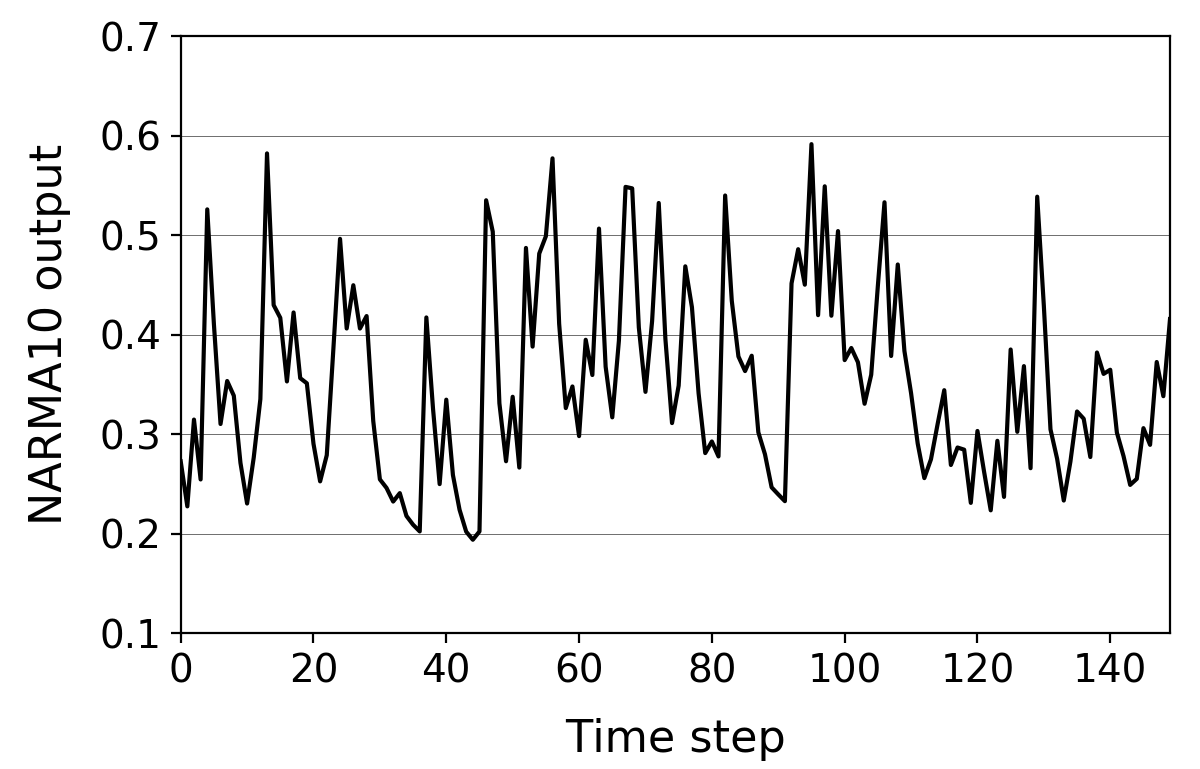
\includegraphics[width=3.0in]{figures/NARMA10.png}
  \caption{
    Example output generated by a 10th-order NARMA system. The autoregressive
moving average nature of the time series is clearly visible.
  }
  \label{narma10-fig}
\end{figure}

The class of time series provided by a nonlinear autoregressive moving average,
most often simply referred to as \textit{NARMA}, is a model commonly used to
benchmark recurrent networks \cite{atiya_new_2000}. Its widespread use yields
baseline performances for well established models, as well as more novel
approaches \cite{verstraeten_experimental_2007, appeltant_information_2011}.

NARMA provides discrete-time temporal tasks, introducing a time-lag of $n$ time
steps, and is given by

\begin{equation}
  y_{t} = \alpha y_{t-1} +
  \beta y_{t-1} \sum_{i=1}^{n}y_{t-i} +
  \gamma u_{t-1}u_{t-n} +
  \delta.
  \label{narma-eq}
\end{equation}

Here, $n$ is the order of the system, and common constant parameters are $\alpha
= 0.3$, $\beta = 0.05$, $\gamma = 1.5$ and $\delta = 0.1$. The input $u_{t}$ is
an i.i.d. stream drawn uniformly from the interval [0, 0.5]. The time series is
unstable, and tasks with higher than a 10th-order time lag introduce a
saturation function to produce a bounded sequence:

\begin{equation}
  y_{t} =
  \tanh(
  \alpha y_{t-1} +
  \beta y_{t-1} \sum_{i=1}^{n}y_{t-i} +
  \gamma u_{t-1}u_{t-n} +
  \delta
  ).
  \label{narma-tanh-eq}
\end{equation}

Predicting a NARMA time series, given an input sequence $u$, presents a
challenge of both memory and nonlinearity. This makes NARMA well-suited for
evaluating both the memory capacity and computational power of reservoirs with a
single metric. Reservoirs must necessarily remember input sequences of length
$n$, and should preferably adhere to suitable dynamics on top of this. A 10th-order system is depicted in Figure \ref{narma10-fig}

Evaluation of ESN performance on the NARMA10 system is a thoroughly explored
area in the field of RC. Reported NRMSE performances for traditional ESN
reservoirs of size $N = 200$ lie in the range [0.20, 0.25]
\cite{verstraeten_experimental_2007, goudarzi_comparative_2014,
rodan_minimum_2011, jaeger_adaptive_2003}. For some context, using a shift
register containing the input as a reservoir will achieve a minimal NRMSE of
0.4. To achieve NRMSE values below this threshold it is necessary to introduce
nonlinearity in the reservoir.

%%% Local Variables:
%%% mode: latex
%%% TeX-master: "../thesis"
%%% End: